\section{Yêu cầu của hệ thống}
\subsection{Mục tiêu chi tiết của đề tài}
%lợi ích thực tế của giải pháp được đề xuất
Đồ án hướng tới mục tiêu hiện thực một mô-đun nhận diện khuôn mặt có khả năng tích hợp linh hoạt vào các hệ thống hiện có, cung cấp một giải pháp linh hoạt cho nhiều bối cảnh ứng dụng và đa dạng nền tảng phần cứng. Trong bối cảnh nhu cầu thực tiễn ngày càng gia tăng - điển hình như các hệ thống chấm công và truy cập\cite{17_10128985} - đồng thời số lượng nghiên cứu và giải pháp trên vi điều khiển vẫn còn khiêm tốn\cite{35_10457480}, đề tài được định hướng nhằm góp phần thúc đẩy phát triển lĩnh vực nhận diện khuôn mặt trên các thiết bị tài nguyên giới hạn, đặc biệt là các hệ thống nhúng vi xử lý 32-bit. 

Bên cạnh đó, thông qua quá trình thiết kế và triển khai, đồ án kỳ vọng rút ra các kết luận thực nghiệm về hiệu quả của các kỹ thuật nén mô hình, qua đó làm rõ mối quan hệ đánh đổi giữa độ chính xác và chi phí tài nguyên khi triển khai học sâu trên phần cứng hạn chế. Đồng thời, hệ thống được kỳ vọng cung cấp một quy trình hướng dẫn chi tiết, bao quát từ giai đoạn thiết kế mô hình đến triển khai thực tế trên thiết bị.

Với các mục tiêu trên, hệ thống được đặt ra một số yêu cầu cốt lõi. Trước hết, hệ thống cần đạt độ chính xác cao trong các môi trường tính toán mạnh, đồng thời duy trì khả năng chuyển đổi linh hoạt sang các phiên bản tối ưu hóa gọn nhẹ, phù hợp triển khai trên phần cứng nhúng có tài nguyên hạn chế, mà không làm suy giảm đáng kể hiệu năng. Đồng thời, hệ thống cần duy trì độ chính xác ổn định ngay cả trong các môi trường không kiểm soát (như biến thiên ánh sáng, góc chụp, che khuất,$\ldots$), nhằm đảm bảo tính khả thi và giá trị ứng dụng thực tiễn của đề tài.

Do đặc thù của các hệ thống xác thực, độ chính xác là tiêu chí then chốt, trong đó cần đặc biệt hạn chế tối đa các trường hợp chấp nhận sai (false acceptance rate) nhằm giảm thiểu rủi ro về an ninh và tài sản. Song song đó, hệ thống cũng phải đảm bảo trải nghiệm người dùng tự nhiên và thuận tiện, tránh tỷ lệ từ chối sai (false rejection rate) cao gây gián đoạn trong các kịch bản sử dụng thường xuyên như nhà thông minh.

Bên cạnh đó, hệ thống cần được thiết kế theo hướng cho phép mở rộng linh hoạt để tích hợp các chức năng nâng cao như phát hiện tấn công giả mạo (anti-spoofing), cũng như dễ dàng điều chỉnh để phù hợp với các bối cảnh triển khai cụ thể. Cuối cùng, khả năng tương thích và tích hợp với các hệ thống quản lý danh tính và kiểm soát truy cập hiện có cũng là một yêu cầu quan trọng nhằm đảm bảo tính ứng dụng thực tiễn. 

Chi tiết các yêu cầu hệ thống được trình bày sau đây:
\subsection{Yêu cầu chức năng}
\begin{enumerate}
    \item Hệ thống có khả năng thu nhận hình ảnh thông qua camera.
    \item Hệ thống tiếp nhận yêu cầu xác thực và thông tin danh tính từ người dùng và thực hiện xác thực danh tính người dùng dựa trên hình ảnh khuôn mặt đã thu nhận và trả về thông tin xác thực.
    \item Hệ thống cho phép đăng ký người dùng mới bằng cách thu nhận và lưu trữ đặc trưng khuôn mặt vào kho dữ liệu thư viện.
    \item Hệ thống hỗ trợ chức năng xóa bỏ khuôn mặt người dùng khỏi kho dữ liệu thư viện khi không còn nhu cầu sử dụng hoặc khi có yêu cầu cập nhật thông tin xác thực.
\end{enumerate}

\subsection{Yêu cầu phi chức năng}
\begin{enumerate}
    \item Hệ thống phải đảm bảo thời gian đáp ứng không vượt quá 1 giây kể từ thời điểm nhận yêu cầu xác thực khuôn mặt.
    \item Hệ thống phải đạt độ chính xác tối thiểu 95\% trong các điều kiện môi trường được kiểm soát và tối thiểu 90\% trong các điều kiện không kiểm soát.
    \item Tỷ lệ chấp nhận nhầm (FAR) của hệ thống phải không vượt quá 3\% trong các điều kiện môi trường được kiểm soát và không vượt quá 5\% trong các điều kiện có biến thiên về ánh sáng.
    \item Tỷ lệ từ chối nhầm (FRR) của hệ thống phải không vượt quá 10\% trong cả hai kịch bản môi trường nêu trên.
    \item Hệ thống phải có khả năng triển khai và vận hành trên ít nhất một thiết bị nhúng vi điều khiển 32-bit đồng thời đảm bảo các yêu cầu phi chức năng trên cũng như ràng buộc tài nguyên của phần cứng.
    \item Hệ thống cần được thiết kế theo hướng mô-đun hóa nhằm hỗ trợ tích hợp, mở rộng và tùy biến dễ dàng theo các yêu cầu triển khai cụ thể.
\end{enumerate}

\subsection{Phân tích yêu cầu hệ thống}
Đối với các yêu cầu kỹ thuật đã nêu, tồn tại nhiều đánh đổi quan trọng trong quá trình thiết kế hệ thống. Trước hết là đánh đổi giữa khả năng triển khai trên thiết bị nhúng và độ chính xác. Với các ràng buộc về tài nguyên như tần số xử lý và dung lượng bộ nhớ, mô hình cần được thiết kế cân bằng giữa kích thước, số lượng tham số và năng lực biểu diễn đặc trưng. Đồng thời, do các hệ thống nhúng thường hoạt động trong bối cảnh thời gian thực, độ trễ suy luận trở thành một tiêu chí quan trọng. Các yếu tố như memory footprint, tập phép toán được hỗ trợ trên phần cứng, cùng với các kỹ thuật nén mô hình cần được xem xét đồng thời nhằm lựa chọn được kiến trúc phù hợp.

Một đánh đổi khác mang tính bản chất trong các hệ thống xác thực là giữa tỷ lệ chấp nhận nhầm (False Acceptance Rate - FAR) và tỷ lệ từ chối nhầm (False Rejection Rate - FRR). Do đó, hệ thống cần được hiệu chỉnh ngưỡng quyết định một cách hợp lý để đạt được sự cân bằng giữa yêu cầu an ninh và trải nghiệm người dùng.

Ngoài ra, bối cảnh triển khai cũng ảnh hưởng đáng kể đến hiệu năng mô hình. Sự biến thiên các yếu tố môi trường có thể gây suy giảm độ chính xác nếu không được xem xét trong quá trình thiết kế và đánh giá. Vì vậy, phạm vi nghiên cứu của đề tài giả định các biến thiên này ở mức thực tế, bao gồm biến thiên điều kiện ánh sáng, góc chụp và biểu cảm khuôn mặt, nhằm mô phỏng môi trường vận hành của các hệ thống kiểm soát truy cập - một trong những ứng dụng tiêu biểu của bài toán xác thực khuôn mặt nói riêng và nhận diện khuôn mặt nói chung.
\section{Thiết kế hệ thống}
\subsection{Kiến trúc hệ thống}
\begin{figure}[ht]
  \centering
  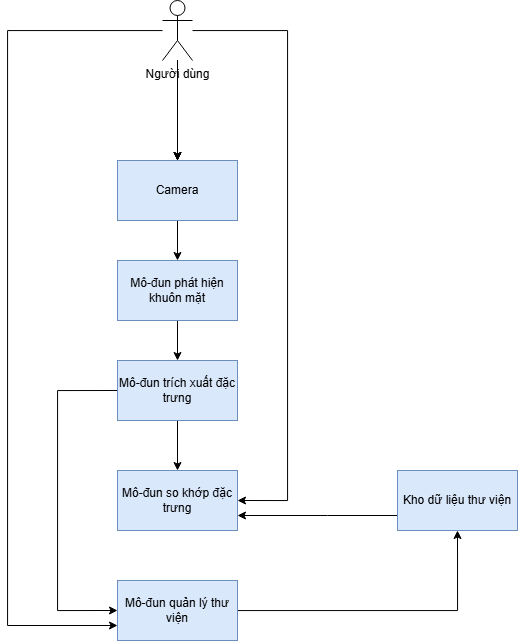
\includegraphics[width=0.5\linewidth]{images/Architecture.drawio.png}
  \caption{Kiến trúc hệ thống xác minh khuôn mặt}
  \label{fig:architecture}
\end{figure}
Về tổng thể, kiến trúc hệ thống xác minh khuôn mặt (Hình \ref{fig:architecture}) được xây dựng theo chuỗi xử lý chuẩn, bao gồm các mô-đun chính: phát hiện và căn chỉnh khuôn mặt, trích xuất đặc trưng, so khớp đặc trưng và quản lý thư viện. Nhằm đáp ứng yêu cầu triển khai trên thiết bị tài nguyên hạn chế, toàn bộ các mô-đun được thiết kế để vận hành tại biên, hạn chế phụ thuộc vào kết nối không dây do các tác vụ giao tiếp (ví dụ thông qua WiFi) làm gia tăng tiêu thụ năng lượng và chi phí bộ nhớ.

Để đảm bảo tính khả thi trong phạm vi đồ án, hệ thống tập trung hiện thực tập chức năng tối thiểu cần thiết, đồng thời vẫn giữ được tính hoàn chỉnh của pipeline xử lý. Bên cạnh đó, kiến trúc được tổ chức theo hướng mô-đun hóa, với các mô-đun có chức năng tách biệt và interface được định nghĩa rõ ràng, qua đó tạo điều kiện thuận lợi cho việc tích hợp, mở rộng và tùy biến trong các hệ thống hiện có.
\subsubsection{ Mô tả các thành phần chức năng}

Người dùng là đối tượng tương tác trực tiếp với hệ thống, xuất hiện trước camera cũng như cung cấp thông tin định danh để thực hiện quá trình xác thực danh tính. Trong một số trường hợp, người dùng cũng có thể đóng vai trò quản trị viên thông qua mô-đun quản lý thư viện khuôn mặt.

Camera có nhiệm vụ thu nhận hình ảnh khuôn mặt từ môi trường thực và cung cấp dữ liệu đầu vào cho các mô-đun xử lý phía sau. Camera có thể là camera tích hợp trên thiết bị nhúng hoặc camera rời, tùy thuộc vào kịch bản triển khai.

Mô-đun phát hiện khuôn mặt thực hiện việc xác định vị trí khuôn mặt trong ảnh đầu vào và loại bỏ các vùng không liên quan, đồng thời có thể căn chỉnh dữ liệu đầu vào cho bước trích xuất đặc trưng. Đầu ra của mô-đun là ảnh khuôn mặt đã được cắt và căn chỉnh.

Mô-đun trích xuất đặc trưng chuyển đổi ảnh khuôn mặt sang dạng vector đặc trưng trong không gian đặc trưng có số chiều xác định. Các vector này được thiết kế sao cho có khả năng phân biệt cao giữa các cá thể khác nhau, đồng thời giảm thiểu sự biến thiên nội lớp.

Mô hình so khớp đặc trưng đảm nhiệm việc so khớp vector đặc trưng đầu vào với vector đặc trưng tương ứng với danh tính đã được lưu trữ trong kho dữ liệu khuôn mặt để đưa ra kết luận chấp nhận hay không.

Kho dữ liệu thư viện khuôn mặt lưu trữ các vector đặc trưng của những người đã được đăng ký cùng với các thông tin định danh liên quan. Kho dữ liệu này đóng vai trò trung tâm trong quá trình truy vấn và cập nhật thông tin khuôn mặt.

Mô-đun quản lý thư viện cho phép thêm mới, cập nhật hoặc xóa dữ liệu khuôn mặt trong kho thư viện. Mô-đun này hỗ trợ việc mở rộng tập người dùng và duy trì tính nhất quán của dữ liệu theo thời gian.
\subsubsection{Luồng hoạt động của hệ thống}
\begin{figure}[ht]
  \centering
  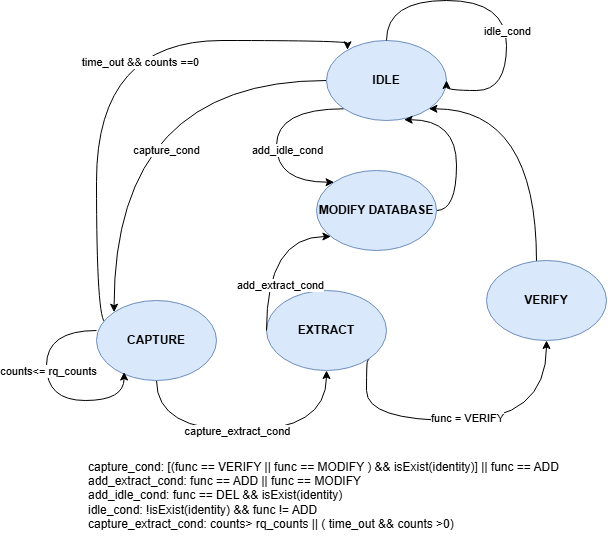
\includegraphics[width=0.5\linewidth]{images/Architecture-StateDiagram.drawio.png}
  \caption{State machine của hệ thống xác minh khuôn mặt}
  \label{fig:state_machine}
\end{figure}
Quy trình hoạt động của hệ thống (được mô tả dưới dạng state machine trong Hình \ref{fig:state_machine}) được tổ chức như sau. Khi người dùng yêu cầu xác thực, hệ thống trước tiên kiểm tra sự tồn tại của định danh trong thư viện. Nếu định danh hợp lệ, hình ảnh được thu nhận liên tục từ camera và chuyển đến mô-đun phát hiện khuôn mặt. Khi khuôn mặt được phát hiện, quá trình ghi hình được tạm dừng, dữ liệu khuôn mặt được căn chỉnh và đưa vào mô-đun trích xuất đặc trưng để sinh ra vector đặc trưng tương ứng. Vector này sau đó được chuyển đến mô-đun so khớp, nơi thực hiện đối sánh với dữ liệu lưu trữ và đưa ra quyết định chấp nhận hoặc từ chối.

Đối với chức năng quản lý thư viện khuôn mặt (bao gồm thêm, xóa, chỉnh sửa), quy trình được thực hiện theo hướng tương tự. Khi có yêu cầu thêm mới hoặc cập nhật dữ liệu hợp lệ, hình ảnh khuôn mặt được thu nhận và xử lý tuần tự qua các mô-đun phát hiện, căn chỉnh và trích xuất đặc trưng. Sau khi hoàn tất, vector đặc trưng được chuyển đến mô-đun quản lý thư viện để thực hiện thao tác lưu trữ hoặc cập nhật. Trong trường hợp xóa dữ liệu, hệ thống sẽ kiểm tra định danh và loại bỏ các vector đặc trưng tương ứng khỏi cơ sở dữ liệu.
\subsection{Thiết bị phần cứng và dụng cụ triển khai}
\subsubsection{Thiết bị phần cứng}
Để đánh giá khả năng triển khai đa nền tảng, đồng thời phù hợp với phạm vi và khối lượng công việc của đồ án, hai dạng nền tảng phần cứng chính sau đây được lựa chọn:

\begin{itemize}
    \item \textbf{Máy tính đa dụng}: Với cấu hình vượt trội về CPU, RAM và khả năng lưu trữ, nền tảng này phù hợp cho các tác vụ yêu cầu hiệu năng cao như xử lý dữ liệu, mô phỏng, lập trình và huấn luyện mô hình học sâu. Việc triển khai trên máy tính đa dụng cho phép đánh giá hiệu năng tối đa của mô hình trong điều kiện tài nguyên đầy đủ, từ đó làm cơ sở tham chiếu cho các bước tối ưu hóa sau này.
    
    \item \textbf{Mạch vi điều khiển 32-bit}: So với các vi điều khiển 8-bit, MCU 32-bit cung cấp năng lực tính toán cao hơn, đủ khả năng thực thi các mô hình học sâu khi được tối ưu hóa phù hợp. Đây cũng là nền tảng phần cứng có chi phí thấp, tiêu thụ năng lượng thấp và linh hoạt trong triển khai thực tế. Đồng thời, hệ sinh thái công cụ ngày càng hoàn thiện, với các framework hỗ trợ như TFLite Micro và Edge Impulse, tạo điều kiện thuận lợi cho việc triển khai mô hình. Với những hạn chế đáng kể về tốc độ xử lý và bộ nhớ trên chip so với các thiết bị di động hiện đại, việc triển khai trên MCU đóng vai trò minh họa rõ ràng cho tính khả thi của mô hình trong các môi trường tài nguyên hạn chế.
\end{itemize}
Trên cơ sở khảo sát tổng quan, kết hợp với các tiêu chí về khả năng tiếp cận và chi phí, nền tảng phần cứng tương ứng được lựa chọn như sau:
\begin{itemize}
    \item Máy tính cá nhân ASUS VivoBook 15 OLED\cite{asus_2023_asus} được trang bị bộ xử lý kiến trúc Intel x64 với xung nhịp 2.60 GHz, bộ nhớ RAM 16 GB và vận hành trên hệ điều hành Windows 64-bit. Thiết bị thu nhận hình ảnh là webcam tích hợp sẵn, hỗ trợ độ phân giải 1280 × 720 @ 30 fps
    \item Module ESP32-CAM Ai-Thinker\cite{aithinker_2020_esp32cam} tích hợp camera OV2640 độ phân giải 2 MP, hỗ trợ tối đa 1600 × 1200 @ 15 fps. Thiết bị sử dụng module trung tâm Ai-Thinker ESP32-S có bộ xử lý Dual-core 32-bit Xtensa LX6 với tần số xung nhịp lên đến 240 MHz; bộ nhớ SRAM trong 520 kB, kết hợp với 4 MB PSRAM ngoài phục vụ cho việc cấp phát dữ liệu trong quá trình thực thi. Ngoài ra, bộ nhớ SPI Flash 4 MB được sử dụng để lưu trữ chương trình và các mô hình học sâu triển khai trên thiết bị.
     \item Hệ sinh thái tích hợp bao gồm một máy chủ s-2vcpu-4gb của DigitalOcean\cite{digitalocean_2026_digitalocean}, được trang bị 2 Intel vCPU, 4 GB RAM và vận hành trên hệ điều hành Ubuntu 24.04 LTS (x64); cùng với thiết bị đầu cuối là máy tính bảng Samsung Galaxy Tab A9\cite{samsung_2023_galaxy}, sở hữu bộ xử lý tám nhân với xung nhịp tối đa 2.2 GHz và 4 GB RAM được trang bị camera hỗ trợ tối đa 1920 x 1080 @ 30fps. Các thành phần trong hệ thống giao tiếp với nhau thông qua giao thức RESTful API, đảm bảo khả năng trao đổi dữ liệu linh hoạt và mở rộng.
\end{itemize}
\subsubsection{Dụng cụ triển khai}
Để hỗ trợ triển khai trên đa nền tảng, đồ án sử dụng hệ sinh thái TensorFlow, trong đó TensorFlow Lite for Microcontrollers (TFLite Micro) được lựa chọn cho các thiết bị nhúng. Cụ thể, quá trình phát triển được thực hiện bằng Python trên các máy tính đa dụng, trong khi phần triển khai trên thiết bị nhúng được hiện thực bằng C/C++.

Hệ sinh thái TensorFlow đóng vai trò then chốt trong quy trình phát triển Tiny Deep Learning, cung cấp chuỗi công cụ toàn diện từ huấn luyện đến triển khai. Các công cụ này bao gồm chuyển đổi mô hình sang định dạng FlatBuffer (.tflite), hỗ trợ các kỹ thuật nén như cắt tỉa và lượng tử hóa, cũng như các công cụ phân tích và thực thi mô hình. Đặc biệt, TFLite Micro cung cấp một lõi suy luận nhẹ, không phụ thuộc hệ điều hành và không sử dụng cấp phát bộ nhớ động, qua đó hạn chế phân mảnh bộ nhớ và phù hợp với các vi điều khiển có tài nguyên hạn chế về RAM và Flash. Nhờ hệ sinh thái phát triển hoàn thiện, tài liệu phong phú và cộng đồng hỗ trợ rộng lớn, TensorFlow đã trở thành một nền tảng tiêu chuẩn (de facto) trong lĩnh vực TinyML, đặc biệt cho các bài toán triển khai học sâu trên thiết bị nhúng.\cite{1_warden_2020_tinyml,14_10.1145/3776588}

\subsection{Lựa chọn công nghệ}
%Biện luận công nghệ, đưa ra 2 option -> thực hiện kiểm chứng
\subsubsection{Mô-đun phát hiện khuôn mặt}
Để hỗ trợ quá trình xác thực khuôn mặt theo thời gian thực, đồng thời giảm thiểu độ phức tạp trong quá trình hiện thực hệ thống, đồ án lựa chọn sử dụng thư viện MediaPipe của Google cho bài toán phát hiện khuôn mặt. Việc lựa chọn này xuất phát từ các ưu điểm nổi bật của MediaPipe như tính đa nền tảng, thời gian suy luận nhanh, cùng với kích thước mô hình gọn nhẹ, phù hợp với yêu cầu triển khai trên các thiết bị có tài nguyên phần cứng hạn chế và các hệ thống nhúng.

Mô hình phát hiện khuôn mặt của MediaPipe có thể hoạt động trên cả ảnh tĩnh và luồng video liên tục (image stream). Kết quả đầu ra bao gồm vị trí khuôn mặt dưới dạng bounding box và tập các điểm mốc đặc trưng trên khuôn mặt, chẳng hạn như mắt, đỉnh mũi, miệng và điểm tragion, từ đó tạo điều kiện thuận lợi cho các bước xử lý tiếp theo như trích xuất đặc trưng và xác thực danh tính.

Đặc biệt, MediaPipe cung cấp nhiều biến thể mô hình tương ứng với các khoảng cách phát hiện và kích thước ảnh khác nhau. Trong đó, mô hình BlazeFace full-range được tối ưu cho các nguồn ảnh như camera sau hoặc webcam, và được cung cấp dưới hai phiên bản. Cả hai biến thể, BlazeFace tiêu chuẩn và BlazeFace Sparse\cite{bazarevsky2019blazeface}, đều là các mạng tích chập với kiến trúc tương tự CenterNet, được thiết kế cho bài toán phát hiện khuôn mặt thời gian thực trên thiết bị di động, tuy nhiên khác biệt đáng kể về mức độ tối ưu hóa và hiệu năng.

Về cấu trúc, BlazeFace tiêu chuẩn có kích thước khoảng 1,1 MB, trong khi phiên bản Sparse được giảm xuống còn khoảng 680 KB nhờ áp dụng kỹ thuật pruning, loại bỏ khoảng 70\% trọng số trong các lớp tích chập 1×1. Nhờ đó, BlazeFace Sparse đạt tốc độ suy luận cao hơn trên CPU (khoảng 160 FPS so với 145 FPS trên Pixel 4), trong khi hiệu năng trên GPU gần như tương đương giữa hai phiên bản. Tuy nhiên, sự tinh giản này đi kèm với suy giảm nhẹ về độ chính xác: BlazeFace tiêu chuẩn đạt recall và precision trung bình trên toàn cầu khoảng 99,3\% và 89,3\%, trong khi phiên bản Sparse giảm xuống lần lượt còn 98,8\% và 82,9\%.

Vì vậy, trong phạm vi đồ án với mục tiêu triển khai trên vi điều khiển có bộ nhớ Flash hạn chế (4 MB), phiên bản BlazeFace Sparse là lựa chọn phù hợp hơn nhờ kích thước nhỏ và tốc độ xử lý cao, dù chấp nhận một mức suy giảm nhất định về độ chính xác.
\subsubsection{Mô-đun trích xuất đặc trưng}
\paragraph{Kiến trúc mô hình học sâu}

Với các hạn chế về tài nguyên tính toán trong giai đoạn huấn luyện, đồ án lựa chọn hướng tiếp cận transfer learning kết hợp với nén mô hình trên các mô hình tiền huấn luyện (pretrained models). Nhằm đảm bảo khả năng triển khai hiệu quả trên các nền tảng tài nguyên hạn chế, một số kiến trúc phù hợp đã được khảo sát tại Bảng \ref{tab:my_architecture}
\begin{table}[]
    \centering
    \small
    \begin{tabular}{|p{5cm}|c|c|}
        \hline
         \textbf{Tên}& \textbf{Kích thước (MB)} & \textbf{Độ chính xác trên LFW(\%)}  \\
         \hline
         MobileFaceNet\cite{16_chen_2018_mobilefacenets}& 4.0 & 99.55 \\
         MobiFace\cite{ARC_9185981} & 9.3 & \textbf{99.71}\\
         Squeezenet with GDC\cite{41_8939565} & 6.2 & 99.05\\ 
         ShuffleFaceNet 1x \cite{42_Martindez-Diaz_2019_ICCV}& 5.6 & 99.45 \\
         ShuffleFaceNet 0.5x \cite{42_Martindez-Diaz_2019_ICCV}& \textbf{1.9} & 99.23 \\
         \hline
    \end{tabular}
    \caption{Bảng so sánh các kiến trúc gọn nhẹ trong bài toán nhận diện khuôn mặt}
    \label{tab:my_architecture}
\end{table}

Mặc dù MobiFace đạt độ chính xác cao và ShuffleFaceNet 0.5× có kích thước nhỏ nhất, MobileFaceNet được lựa chọn làm kiến trúc nền tảng nhằm cân bằng giữa độ chính xác và khả năng triển khai thực tế trên nền tảng ESP32-CAM, đồng thời được hỗ trợ bởi nguồn tài nguyên mã nguồn mở, thuận lợi cho phát triển và triển khai. Trên cơ sở đó, các kỹ thuật nén mô hình phù hợp sẽ được áp dụng nhằm tiếp tục giảm kích thước và chi phí tính toán, đồng thời duy trì hiệu năng ở mức chấp nhận được.
\paragraph{Kỹ thuật nén mô hình}
\begin{figure}[ht]
  \centering
  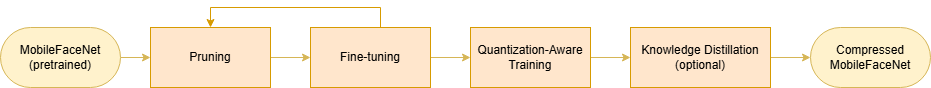
\includegraphics[width=\linewidth]{images/Pipeline.drawio.png}
  \caption{Pipeline nén mô hình MobileFaceNet pretrained}
  \label{fig:compress-pipeline}
\end{figure}
Để nén mô hình, đề tài áp dụng kết hợp các kỹ thuật quantization và pruning, đồng thời sử dụng knowledge distillation (KD) nhằm phục hồi độ chính xác sau quá trình nén. Quy trình tổng thể được trình bày trong Hình \ref{fig:compress-pipeline}. 

Cụ thể, phương pháp iterative structured pruning được lựa chọn với mục tiêu giảm kích thước mô hình khoảng 1.5–2 lần. Do nền tảng ESP32 không hỗ trợ hiệu quả các phép toán trên ma trận thưa, unstructured pruning chủ yếu chỉ giúp giảm dung lượng lưu trữ trên Flash mà không mang lại cải thiện đáng kể về bộ nhớ hoạt động (runtime memory) hay thời gian suy luận. Vì vậy phương pháp kết hợp được sử dụng để tận dụng ưu điểm của cả hai. Trong đó, structured pruning theo tiêu chí magnitude-based - với ưu điểm đơn giản trong triển khai - được áp dụng nhằm loại bỏ các kênh (channels) ít quan trọng trong các tầng trung gian, qua đó giảm kích thước mô hình và memory footprint của các activation maps. Tuy nhiên, quá trình cắt tỉa thường dẫn đến suy giảm độ chính xác, do đó cần thực hiện fine-tuning để phục hồi hiệu năng trước song song với các bước cắt tỉa. Cùng với đó, chiến lược iterative pruning (lặp lại nhiều vòng cắt tỉa và tinh chỉnh) cũng được áp dụng dựa vào quan sát chiến lược trên thường mang lại hiệu quả tốt hơn so với one-shot pruning. Unstructured pruning sẽ được thực hiện dưới dạng global pruning (hay group pruning), tức là nhiều lớp (layers) hoặc module trong mạng sẽ được xem như một khối thống nhất. Thay vì áp dụng tỷ lệ cắt tỉa cố định cho từng lớp riêng lẻ, phương pháp này tiến hành xếp hạng mức độ quan trọng của toàn bộ các tham số trên toàn mạng và loại bỏ các trọng số kém quan trọng nhất theo một ngưỡng chung. Do đó, tỷ lệ cắt tỉa thực tế tại mỗi lớp có thể khác nhau, phản ánh sự phân bố không đồng đều về mức độ quan trọng của các tham số giữa các lớp.\cite{mao_2021_pytorch}

Tiếp theo, mô hình được lượng tử hóa về dạng INT8 nhằm giảm đáng kể kích thước lưu trữ và chi phí tính toán, đồng thời vẫn duy trì độ chính xác ở mức chấp nhận được. Trong cấu hình này, trọng số thường được lượng tử hóa theo kênh (per-channel), trong khi các đặc trưng kích hoạt được lượng tử hóa theo tensor (per-tensor/per-layer) để cân bằng giữa độ chính xác và độ phức tạp triển khai; bias được giữ ở độ chính xác cao hơn (thường là INT32) nhằm hạn chế sai số tích lũy.

Để giảm thiểu suy giảm độ chính xác do lượng tử hóa, phương pháp quantization-aware training (QAT) được áp dụng, cho phép mô hình thích nghi với sai số lượng tử trong quá trình fine-tuning. Cuối cùng, knowledge distillation được xem xét như một bước bổ sung nhằm cải thiện chất lượng biểu diễn của mô hình nén; tuy nhiên, do hiệu quả của KD phụ thuộc vào cấu hình cụ thể, việc áp dụng sẽ được đánh giá thực nghiệm trước khi tích hợp vào pipeline chính thức.

\paragraph{Hàm mất mát}

Hàm mất mát đóng vai trò quan trọng trong việc nâng cao khả năng phân biệt của mô hình mà không làm gia tăng độ phức tạp tính toán tại runtime. Dựa trên các phương pháp đã được khảo sát (Bảng \ref{tab:loss_table}), trong đề tài này lựa chọn sử dụng hàm mất mát ArcFace - một phương pháp tiên tiến (state-of-the-art) trong bài toán nhận dạng khuôn mặt, nhờ khả năng đạt hiệu năng cao đồng thời vẫn dễ dàng triển khai trong thực tế.

ArcFace cải thiện khả năng phân tách đặc trưng bằng cách đưa thêm một biên góc (angular margin) trực tiếp vào không gian embedding đã được chuẩn hóa, từ đó làm tăng khoảng cách giữa các lớp khác nhau (inter-class separation) và đồng thời giảm độ phân tán trong cùng một lớp (intra-class compactness).

\subsubsection{Mô-đun so khớp khuôn mặt}

Tương ứng với quá trình huấn luyện sử dụng ArcFace, độ tương đồng giữa hai khuôn mặt trong giai đoạn suy luận thường được đo bằng cosine similarity, do thước đo này phản ánh trực tiếp khoảng cách góc giữa các vector embedding - đại lượng mà ArcFace tối ưu hóa trong quá trình huấn luyện. Nhờ đó, việc sử dụng cosine similarity đảm bảo tính nhất quán giữa hai giai đoạn huấn luyện và suy luận, trong đó hai khuôn mặt được xem là cùng một danh tính khi góc giữa các vector embedding nhỏ (tương ứng với giá trị cosine lớn).

Tuy nhiên, việc tính toán cosine similarity trên các thiết bị nhúng có thể gây tốn kém chi phí tính toán, đặc biệt khi vector embedding chưa được chuẩn hóa, do cần thực hiện các phép toán dấu phẩy động như căn bậc hai và phép chia. Điều này là một hạn chế trên các nền tảng như ESP32-S, vốn có hỗ trợ FPU nhưng hiệu năng đối với các phép toán này còn hạn chế. Ngược lại, khoảng cách Euclid bình phương $\lVert x - y \rVert^2$ có thể được tính toán hiệu quả hơn do chỉ bao gồm các phép cộng và nhân, tuy nhiên không phản ánh trực tiếp khoảng cách góc nên có thể kém chính xác hơn trong bối cảnh embedding được huấn luyện theo tiêu chí góc.

Do đó, trong đồ án này, cả hai thước đo cosine similarity và khoảng cách Euclid bình phương được triển khai song song. Để giảm chi phí tính toán của cosine similarity, các vector embedding sẽ được chuẩn hóa trước bằng phương pháp xấp xỉ nhanh Fast Inverse Square Root, từ đó cho phép đánh giá và so sánh hiệu năng giữa hai phương pháp trong điều kiện triển khai thực tế trên phần cứng hạn chế

\subsection{Kịch bản kiểm thử}
\begin{figure*}[ht]
    \centering
    \begin{subfigure}[t]{0.33\textwidth}
        \centering
        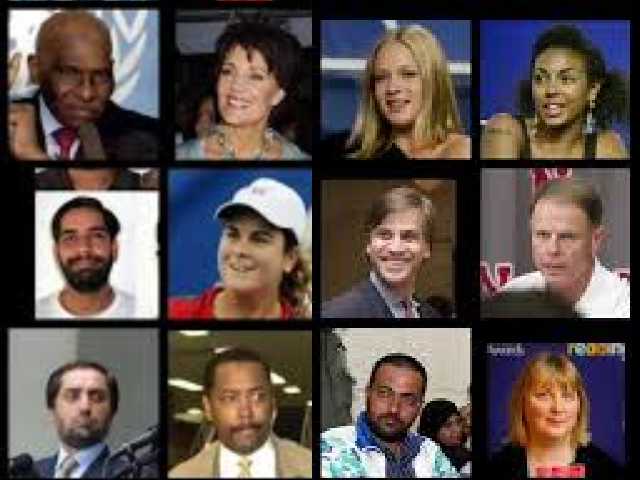
\includegraphics[width=\linewidth]{images/lfw.png}
        \caption{Tập Labeled Faces in the Wild (LFW)}
    \end{subfigure}%
    ~
    \begin{subfigure}[t]{0.33\textwidth}
        \centering
        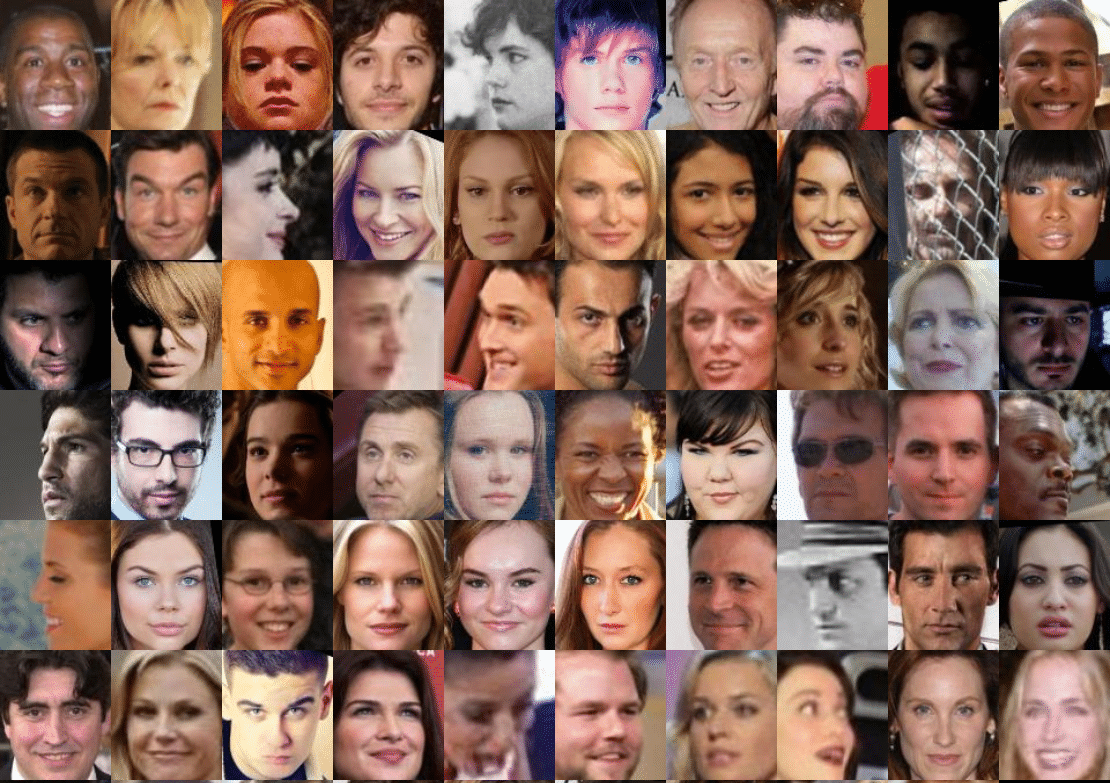
\includegraphics[width=\linewidth]{images/megaface-biometric-facial-recognition-algorithms-testing-datasets.png}
        \caption{Tập MegaFace}
    \end{subfigure}
    ~
    \begin{subfigure}[t]{0.33\textwidth}
        \centering
        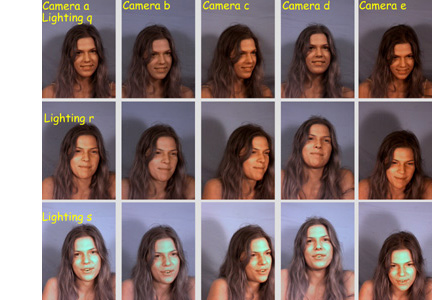
\includegraphics[width=\linewidth]{images/all-simone-images-lores.jpg}
        \caption{Tập MUCT}
    \end{subfigure}
    \label{fig:dataset_used}
    \caption{Các bộ dữ liệu kiểm thử}
\end{figure*}

Với mục tiêu đánh giá toàn diện các yêu cầu phi chức năng của hệ thống, bao gồm độ chính xác, tỷ lệ chấp nhận sai FAR, tỷ lệ từ chối sai FRR, thời gian phản hồi và kích thước mô hình, một kịch bản kiểm thử được đề xuất dựa trên cả môi trường có kiểm soát và không kiểm soát. Để đảm bảo tính đại diện và khả năng so sánh với các nghiên cứu trước, ba bộ dữ liệu chuẩn gồm LFW, MegaFace và MUCT được lựa chọn (Hình \ref{fig:dataset_used})

Tập Labeled Faces in the Wild (LFW)\cite{article} được thiết kế cho bài toán nhận diện khuôn mặt trong điều kiện không kiểm soát. Bộ dữ liệu này bao gồm 13.233 ảnh của 5.749 cá nhân, được thu thập từ các nguồn tự nhiên và xử lý bằng thuật toán phát hiện khuôn mặt Viola–Jones. Trong đó, 1.680 cá nhân có từ hai ảnh trở lên, phù hợp cho các bài toán xác thực.

Tập MegaFace\cite{kemelmachershlizerman2015megafacebenchmark1million} được xây dựng theo hướng mở rộng quy mô, bao gồm hơn 1 triệu ảnh của khoảng 690.000 cá nhân, được thu thập từ nền tảng Flickr. Các khuôn mặt được phát hiện và căn chỉnh bằng thuật toán HeadHunter. Bộ dữ liệu này có tính đa dạng cao về tư thế và điều kiện chụp, với hơn 197.000 ảnh có góc quay đầu lớn, do đó phù hợp để đánh giá hiệu năng hệ thống trong các kịch bản không kiểm soát quy mô lớn.

Tập MUCT\cite{Milborrow2010TheML} là bộ dữ liệu ảnh màu với độ phân giải 480×640, bao gồm 3.755 ảnh khuôn mặt được thu thập trong điều kiện có kiểm soát. Dữ liệu thể hiện sự đa dạng về độ tuổi, chủng tộc và điều kiện chiếu sáng, với các tư thế từ chính diện đến góc nghiêng khoảng 50°. Nhờ các thiết lập thu thập ổn định, MUCT phù hợp để đánh giá hiệu năng hệ thống trong môi trường kiểm soát.

Đối với mô hình đề xuất, quá trình tinh chỉnh tham số được thực hiện trên tập MUCT, tách biệt theo hai module chính: module trích xuất đặc trưng và module nhận diện. Cụ thể, module trích xuất đặc trưng được sử dụng để đánh giá hiệu năng của mô hình dưới các cấu hình nén khác nhau, từ đó lựa chọn cấu hình phù hợp về mặt cân bằng giữa độ chính xác và chi phí tính toán. Đối với module so khớp khuôn mặt, các ngưỡng (threshold) được khảo sát trên hai thước đo tương đồng đề xuất nhằm xác định phương pháp tối ưu cho bài toán xác thực.

Sau khi xác định được bộ tham số tối ưu, hệ thống sẽ được đánh giá toàn diện trên các bộ dữ liệu đã lựa chọn, đồng thời so sánh với các phương pháp tiên tiến (state-of-the-art) nhằm cung cấp cái nhìn khách quan về hiệu quả của phương pháp đề xuất.

\section{Hiện thực đề tài}
\subsection{Thuận lợi}
Về mặt thuận lợi, mô hình MobileFaceNet pretrained được cung cấp dưới nhiều biến thể với sự đa dạng về độ chính xác và kích thước, cho phép lựa chọn cấu hình phù hợp và tiếp tục tinh chỉnh theo yêu cầu của hệ thống. Bên cạnh đó, mặc dù các mô hình này được phát hành dưới nhiều định dạng khác nhau như ONNX hoặc PaddlePaddle, các công cụ chuyển đổi hiện nay đã tương đối hoàn thiện và cho phép chuyển đổi sang định dạng TFLite với độ chính xác cao. Ngoài ra, các tài nguyên đi kèm như mã nguồn và tài liệu hướng dẫn cũng hỗ trợ xác định rõ định dạng, kích thước và dải giá trị đầu vào, từ đó tạo điều kiện thuận lợi cho việc tích hợp và triển khai trên nền tảng mục tiêu.
\subsection{Khó khăn}
\subsubsection{Sự phức tạp của các framework}
Về mặt triển khai, một trong những khó khăn chính của đồ án nằm ở việc hiện thực module phát hiện khuôn mặt. Mặc dù MediaPipe cung cấp sẵn mô hình suy luận dưới dạng tệp TFLite, framework tiền xử lý (preprocessing) và hậu xử lý (postprocessing) công bố bởi MediaPipe lại tương đối phức tạp và không cung cấp hỗ trợ trên thiết bị nhúng. Cụ thể, đầu ra của mô hình bao gồm các tensor dạng mảng, yêu cầu phải thực hiện thêm các bước xử lý như giải mã bounding box dựa trên các anchor và áp dụng thuật toán Non-Maximum Suppression (NMS) để loại bỏ các dự đoán trùng lặp. Việc tái hiện chính xác pipeline này từ đầu gây ra nhiều thách thức trong quá trình triển khai trên thiết bị nhúng. Để khắc phục vấn đề này, tác giả đã tham khảo và sử dụng một dự án mã nguồn mở của patlevin\footnote{https://github.com/patlevin/face-detection-tflite}
, sau đó tiến hành tinh gọn và điều chỉnh dựa trên điều kiện vận hành nhằm phù hợp với yêu cầu tài nguyên và kiến trúc của hệ thống đề xuất. 
\subsubsection{Sự sụt giảm hiệu suất của mô hình khi tự hiện thực}
\begin{figure}[ht]
  \centering
  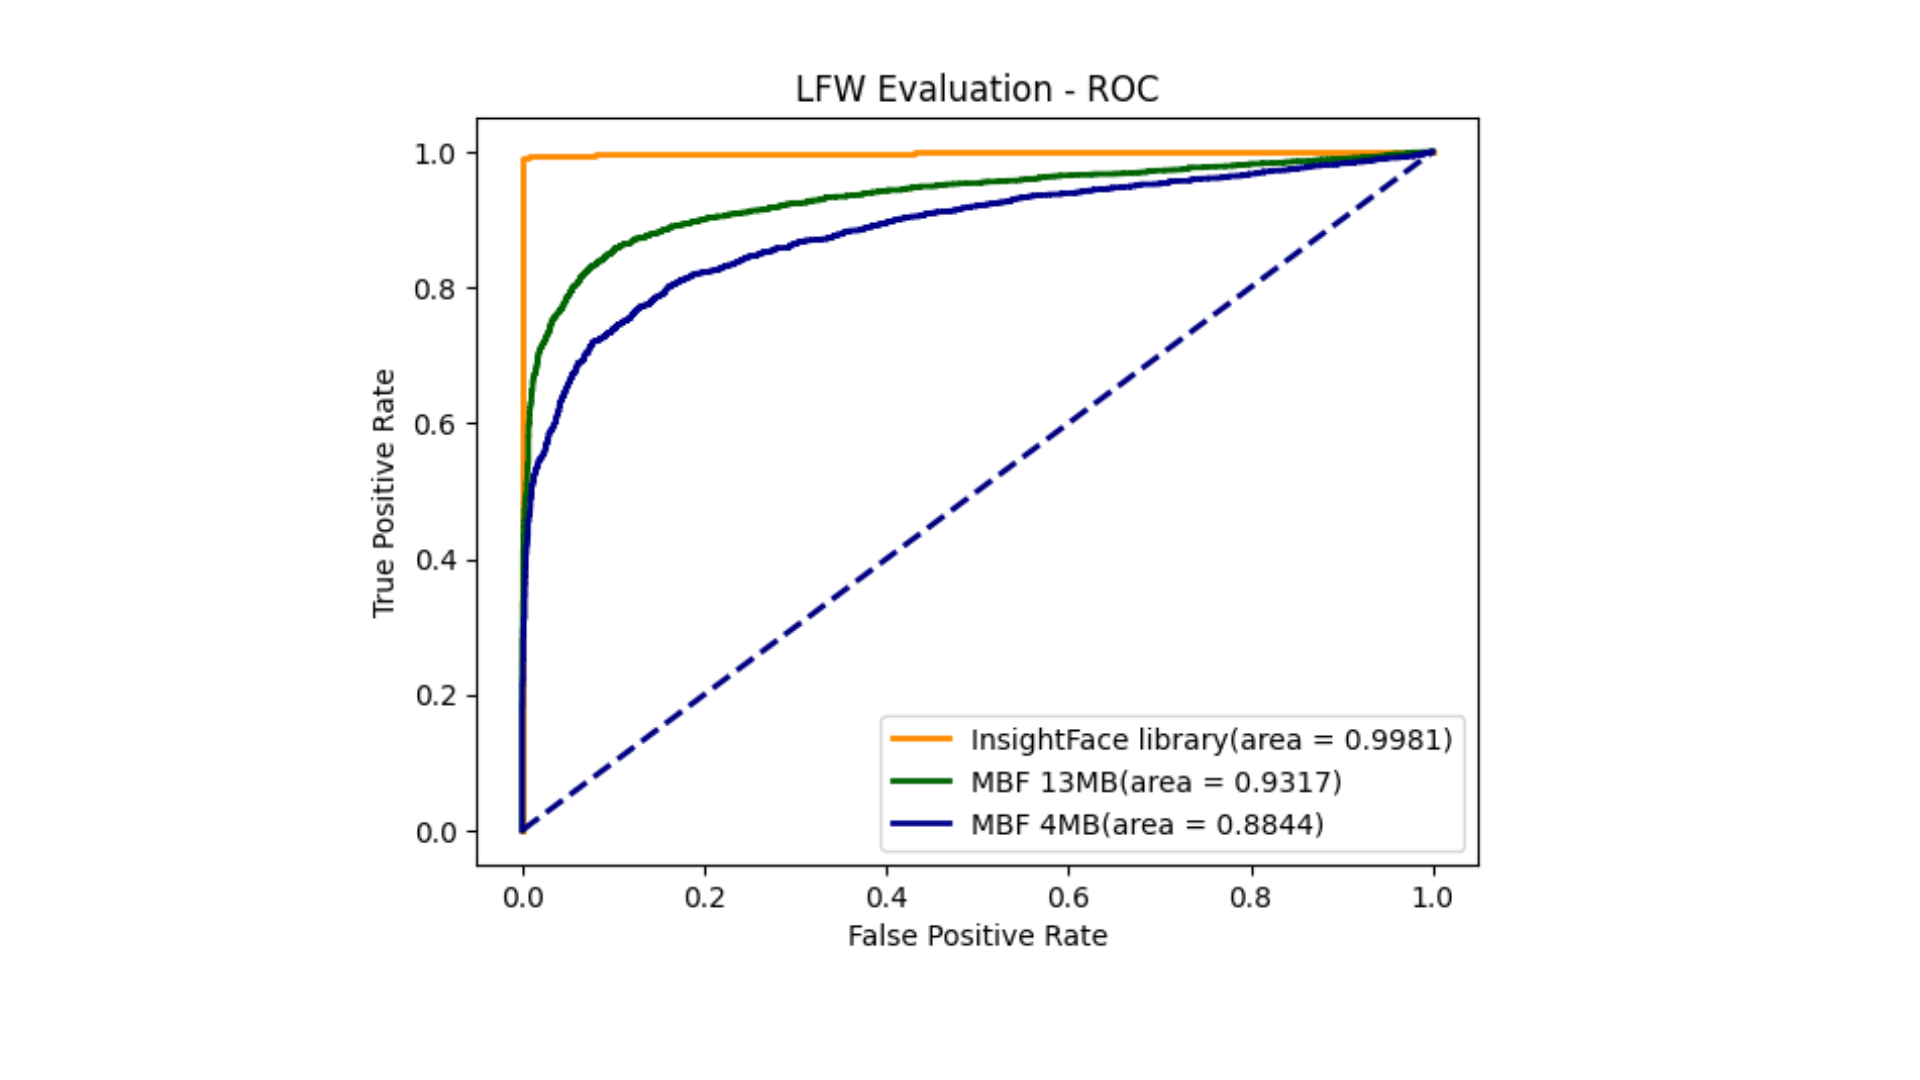
\includegraphics[width=0.5\linewidth]{images/Untitled design.png}
  \caption{Hiệu suất mô hình với cấu hình chưa được tinh chỉnh}
  \label{fig:before}
\end{figure}

Việc thay thế mô hình phát hiện và tái hiện các hàm face alignment từ thư viện gốc đã dẫn đến sự suy giảm đáng kể về hiệu năng, mặc dù các hàm căn chỉnh đã được hiện thực gần tương đương (Hình \ref{fig:before}). Nguyên nhân chủ yếu xuất phát từ sự sai lệch của cấu hình chuẩn trong hệ thống mục tiêu. Cụ thể, thư viện InsightFace thực hiện ánh xạ các điểm mốc (landmarks) do mô hình SCRFD phát hiện sang một cấu hình chuẩn cố định nhằm chuẩn hóa hình học khuôn mặt trước khi trích xuất đặc trưng. Tuy nhiên, do sự khác biệt trong cách xác định và biểu diễn landmark (về số lượng và loại điểm mốc), mô hình phát hiện BlazeFace không thể trực tiếp sử dụng cấu hình chuẩn này và cần một cấu hình chuẩn khác. Việc tự suy ra cấu hình chuẩn từ ảnh đầu vào bất kỳ đã dẫn đến sự thay đổi trong phân bố dữ liệu đầu vào (data distribution shift), gây sai lệch trong không gian embedding và làm suy giảm độ chính xác tổng thể.

Để khắc phục, một ảnh tham chiếu được căn chỉnh bằng pipeline của thư viện gốc, sau đó sử dụng chính mô hình phát hiện BlazeFace để suy ra tập landmark tương ứng; tập landmark này được chọn làm cấu hình chuẩn. Mặc dù cấu hình thu được có thể vẫn sai lệch nhất định so với cấu hình mong đợi bởi mô hình trích xuất đặc trưng, kết quả thực nghiệm cho thấy mức suy giảm hiệu năng đã được giảm đáng kể so với phương pháp naive và nằm trong ngưỡng chấp nhận được (Hình \ref{fig:roc}).
\subsection{Triển khai trên máy tính đa dụng}
Sử dụng ngôn ngữ lập trình Python cùng với các thư viện cơ bản như NumPy, OpenCV và ai-edge-litert, đồ án đã xây dựng thành công một module nhận diện khuôn mặt gọn nhẹ với mức phụ thuộc tối thiểu. Thay vì sử dụng các framework phức tạp như MediaPipe hay InsightFace, hệ thống được phát triển dựa trên các thư viện đơn giản hơn, qua đó tạo điều kiện thuận lợi cho việc chuyển đổi sang C/C++ trong giai đoạn triển khai trên thiết bị nhúng.
\begin{figure*}[ht]
    \centering
    \begin{subfigure}[t]{0.40\textwidth}
        \centering
        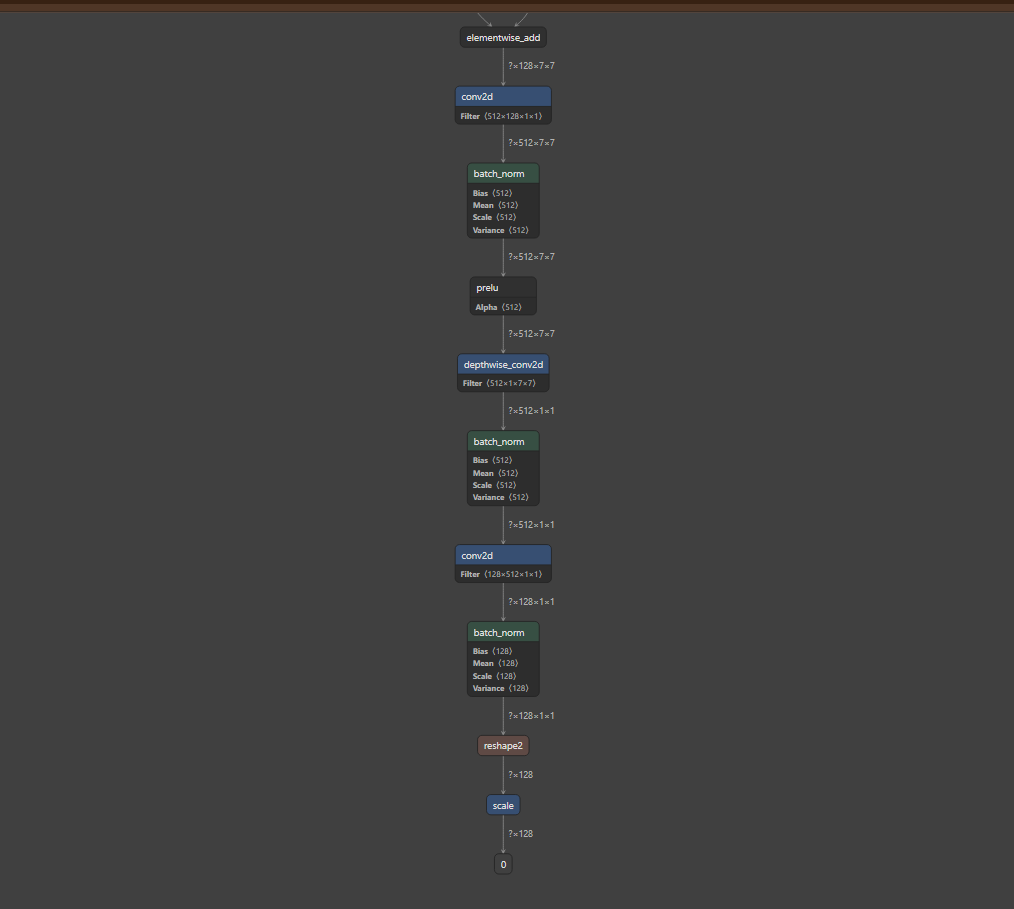
\includegraphics[width=\linewidth]{images/128.png}
        \caption{MBF@WebFace600K - 13MB}
    \end{subfigure}%
    ~
    \begin{subfigure}[t]{0.40\textwidth}
        \centering
        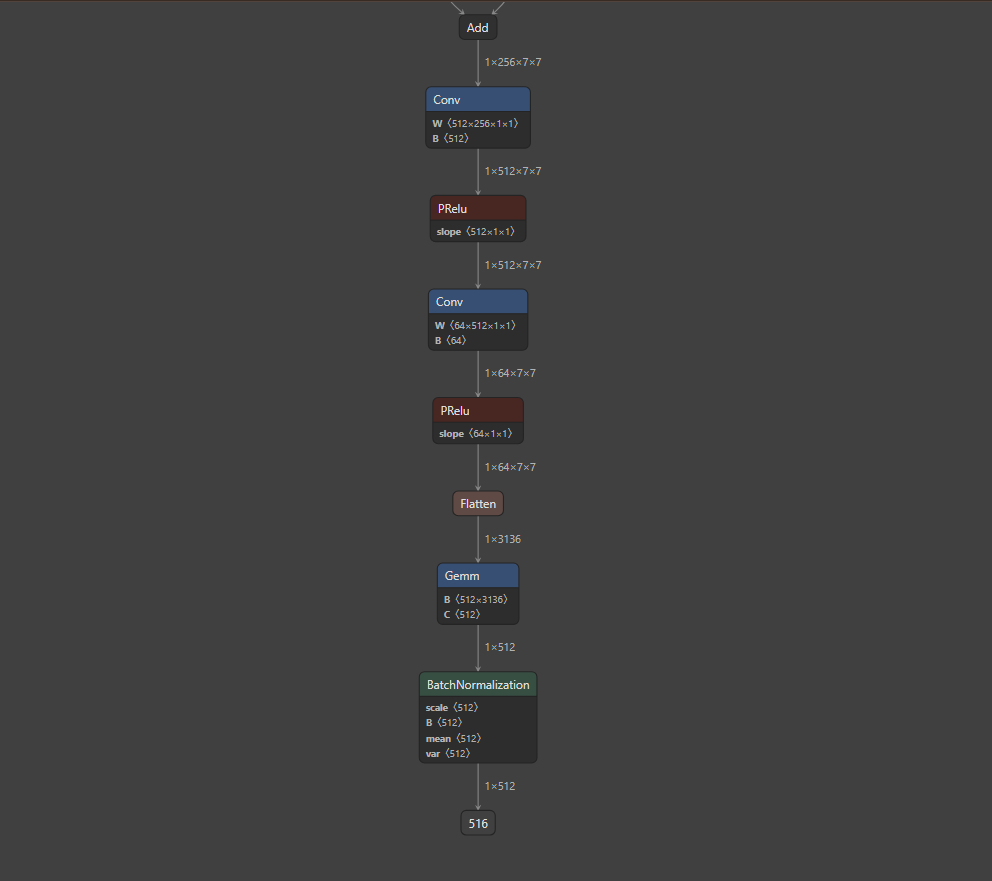
\includegraphics[width=\linewidth]{images/512.png}
        \caption{MBF@MS1MV2 - 4MB}
    \end{subfigure}
    \label{fig:comparision}
    \caption{Kiến trúc các mô hình MobileFaceNet cung cấp bởi InsightFace}
\end{figure*}
InsightFace cung cấp nhiều mô hình pretrained dưới dạng các model pack với cơ chế tải tự động hoặc thủ công, tương ứng với các cấu hình khác nhau về độ chính xác và kích thước. Trong số đó, gói mô hình nhỏ nhất được hỗ trợ trực tiếp bởi thư viện là \texttt{buffalo\_sc}, bao gồm mô hình phát hiện khuôn mặt SCRFD và mô hình trích xuất đặc trưng MobileFaceNet kết hợp với hàm mất mát ArcFace. Tuy nhiên, kích thước của mô hình MobileFaceNet trong cấu hình này lên tới khoảng 13 MB, lớn hơn đáng kể so với kích thước lý thuyết (~4 MB). Nguyên nhân chủ yếu là do việc thay thế lớp Global Depthwise Convolution (GDC) bằng lớp Fully Connected (FC512) ở cuối mạng, đồng thời tăng kích thước vector embedding lên 512 chiều, dẫn đến số lượng tham số tại các lớp cuối tăng lên đáng kể. Đổi lại, cấu hình này đạt độ chính xác cao, lên tới 99.70\% trên tập LFW.

Tuy nhiên, với ràng buộc phần cứng giới hạn khoảng 4 MB Flash, việc tối ưu một mô hình có kích thước lớn như vậy sẽ đòi hỏi chi phí nén và tinh chỉnh đáng kể. Do đó, đồ án lựa chọn một mô hình MobileFaceNet khác cũng được cung cấp bởi InsightFace dưới định dạng PaddlePaddle, có kích thước khoảng 4 MB và đạt độ chính xác 99.45\% trên tập LFW\footnote{https://github.com/deepinsight/insightface/tree/master/model\_zoo}
. Lựa chọn này chấp nhận đánh đổi sự suy giảm về độ chính xác cũng như không được hỗ trợ bởi thư viện hiện tại, nó tạo điều kiện thuận lợi hơn cho các bước nén tiếp theo, đặc biệt trong bối cảnh triển khai trên các thiết bị nhúng có tài nguyên hạn chế.

Kết quả thực nghiệm cho thấy, mặc dù độ chính xác có sự suy giảm nhất định so với các giải pháp dựa trên framework đầy đủ, module đề xuất vẫn đảm bảo khả năng hoạt động ổn định trên máy tính đa dụng, đồng thời đáp ứng tốt các yêu cầu về tính gọn nhẹ và khả năng mở rộng sang môi trường nhúng.


Hệ thống được thiết kế theo hướng đối tượng, trong đó các chức năng chính được đóng gói thành bốn lớp cốt lõi: 
\texttt{Face\_Detection}, \texttt{Face\_Recognition}, \texttt{Feature\_Extraction} và \texttt{Database\_Management}. Mỗi lớp chịu trách nhiệm cho một giai đoạn cụ thể trong pipeline xử lý khuôn mặt, giúp giảm mức độ phụ thuộc giữa các thành phần và hỗ trợ mở rộng hệ thống một cách linh hoạt.
\begin{figure}[ht]
  \centering
  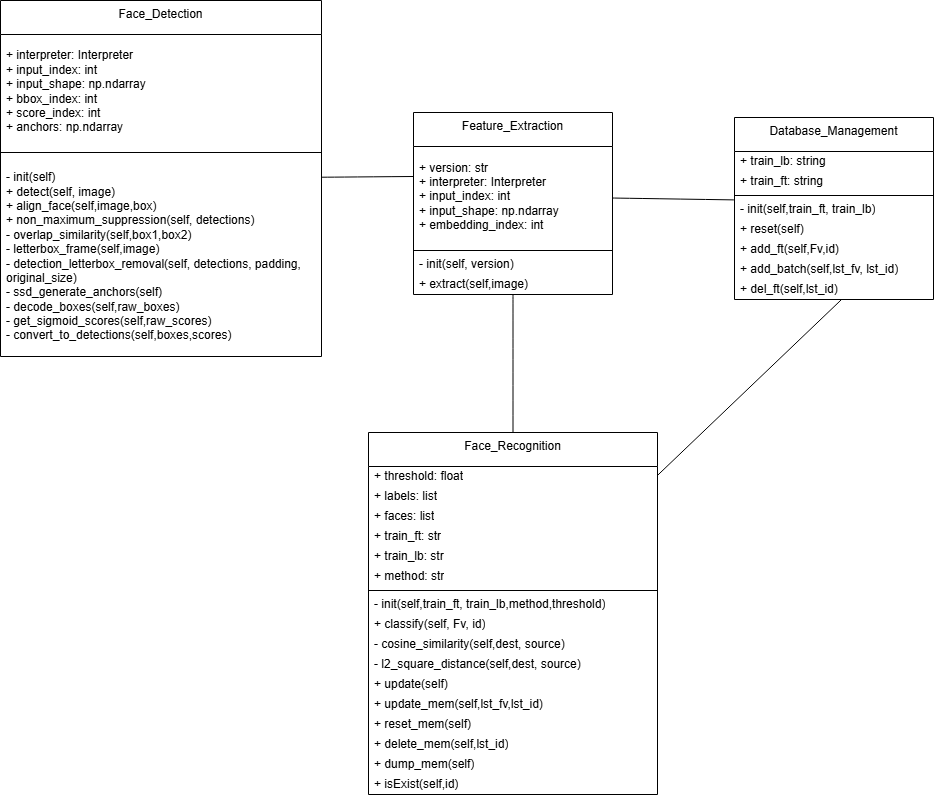
\includegraphics[width=0.75\linewidth]{images/Class Diagram.drawio.png}
  \caption{Sơ đồ lớp của hệ thống xác minh khuôn mặt}
  \label{fig:class_diagrame}
\end{figure}

\subsubsection{Class: \texttt{Face\_Detection}}
\paragraph{Thuộc tính}
\begin{itemize}
    \item \texttt{interpreter} (\texttt{Interpreter}): Đối tượng LiteRT Interpreter dùng để tải mô hình TFLite (MediaPipe) và thực hiện suy luận.
    \item \texttt{input\_index} (\texttt{int}): Chỉ số của tensor đầu vào trong đồ thị suy luận.

    \item \texttt{input\_shape} (\texttt{np.ndarray}): Kích thước của tensor đầu vào, tương ứng với kích thước ảnh đầu vào của mô hình ($1 \times 192 \times 192 \times 3$).

    \item \texttt{bbox\_index} (\texttt{int}): Chỉ số của tensor đầu ra chứa thông tin tọa độ.

    \item \texttt{score\_index} (\texttt{int}): Chỉ số của tensor đầu ra chứa điểm tin cậy (confidence score).

    \item \texttt{anchors} (\texttt{np.ndarray}): Tập các anchor được sử dụng để giải mã các tọa độ từ đầu ra của mô hình.
\end{itemize}
\paragraph{Phương thức}
\begin{itemize}
    \item \texttt{\_\_init\_\_(self)}: Hàm khởi tạo module phát hiện khuôn mặt, bao gồm việc tải mô hình, thiết lập các tham số và khởi tạo các cấu trúc dữ liệu cần thiết.
    
    \item \texttt{detect(self, image)}: Thực hiện phát hiện khuôn mặt trên ảnh đầu vào và trả về danh sách các bounding box kèm theo thông tin landmark.

    \item \texttt{align\_face(self, image, box)}: Căn chỉnh khuôn mặt dựa trên các điểm landmark nhằm chuẩn hóa đầu vào cho module trích xuất đặc trưng.
    
    \item \texttt{non\_maximum\_suppression(self, detections)}: Lọc các kết quả phát hiện bằng cách loại bỏ các bounding box dựa trên độ chồng lấp và điểm tin cậy.
    
    \item \texttt{\_overlap\_similarity(self, box1, box2)}: Tính toán mức độ chồng lấp giữa hai bounding box.
    
    \item \texttt{\_letterbox\_frame(self, image)}: Thực hiện padding để đưa ảnh về kích thước chuẩn mà không làm biến dạng tỉ lệ.
    
    \item \texttt{\_detection\_letterbox\_removal(self, detections, padding, original\_size)}: Loại bỏ ảnh hưởng của padding và ánh xạ lại tọa độ bounding box về kích thước ảnh gốc.
    
    \item \texttt{\_ssd\_generate\_anchors(self)}: Tạo tập các anchor sử dụng trong mô hình phát hiện dựa trên kiến trúc  Single Shot MultiBox Detector (SSD).
    
    \item \texttt{\_decode\_boxes(self, raw\_boxes)}: Giải mã các bounding box từ đầu ra thô của mô hình dựa trên anchor tương ứng.
    
    \item \texttt{\_get\_sigmoid\_scores(self, raw\_scores)}: Áp dụng hàm sigmoid lên các giá trị điểm tin cậy thô (sau khi clipping).
    
    \item \texttt{\_convert\_to\_detections(self, boxes, scores)}: Chuyển đổi các bounding box và điểm tin cậy thành danh sách các đối tượng phát hiện hợp lệ.
\end{itemize}

\subsubsection{Class: \texttt{Feature\_Extraction}}
\paragraph{Thuộc tính}
\begin{itemize}
    \item \texttt{version} (\texttt{str}): Version của model MobileFaceNet được sử dụng
    \item \texttt{interpreter} (\texttt{Interpreter}): Đối tượng LiteRT Interpreter dùng để tải mô hình TFLite và thực hiện suy luận.
    \item \texttt{input\_index} (\texttt{int}): Chỉ số của tensor đầu vào trong đồ thị suy luận.

    \item \texttt{input\_shape} (\texttt{np.ndarray}): Kích thước của tensor đầu vào, tương ứng với kích thước ảnh đầu vào của mô hình ($1 \times 112 \times 112 \times 3$).

    \item \texttt{embedding\_index} (\texttt{int}): Chỉ số của tensor đầu ra chứa đặc trưng được trích xuất.
\end{itemize}
\paragraph{Phương thức}
\begin{itemize}
    \item \texttt{\_\_init\_\_(self, version)}:  Hàm khởi tạo module trích xuất đặc trưng, bao gồm việc tải mô hình, thiết lập các tham số và khởi tạo các cấu trúc dữ liệu cần thiết.
    \item \texttt{extract(self,image)}: hàm trích xuất đặc trưng với kết quả trả về và vector đặc trưng của khuôn mặt thu được mô hình học sâu
\end{itemize}

\subsubsection{Class: \texttt{Face\_Recognition}}
\paragraph{Thuộc tính}
\begin{itemize}
    \item \texttt{faces} (\texttt{list}): Danh sách các vector đặc trưng (embedding) trong cơ sở dữ liệu.
    \item \texttt{labels} (\texttt{list}): Danh sách nhãn định danh tương ứng với từng vector đặc trưng.

    \item \texttt{threshold} (\texttt{float}): Ngưỡng quyết định sử dụng trong module so khớp để quyết định chấp nhận hay không.
    
    \item \texttt{train\_ft} (\texttt{str}): Đường dẫn đến tệp lưu trữ tập đặc trưng khuôn mặt.
    
    \item \texttt{train\_lb} (\texttt{str}): Đường dẫn đến tệp lưu trữ tập nhãn tương ứng.
    
    \item \texttt{method} (\texttt{str}): Phương thức đo độ tương đồng được sử dụng.
\end{itemize}
\paragraph{Phương thức}
\begin{itemize}
    \item \texttt{\_\_init\_\_(self, train\_ft, train\_lb, method, threshold)}: Hàm khởi tạo module so khớp, thực hiện nạp tập đặc trưng và nhãn từ các tệp tương ứng, đồng thời thiết lập phương thức đo độ tương đồng và ngưỡng quyết định.
    \item \texttt{classify(self, Fv, id)}: Thực hiện so khớp vector đặc trưng đầu vào với định danh cho trước và đưa ra quyết định xác thực dựa trên giá trị ngưỡng.
    
    \item \texttt{\_cosine\_similarity(self, dest, source)}: Tính toán độ tương đồng cosine giữa hai vector đặc trưng.
    
    \item \texttt{\_l2\_square\_distance(self, dest, source)}: Tính toán khoảng cách Euclid bình phương giữa hai vector đặc trưng.
    
    \item \texttt{update(self)}: Cập nhật tập dữ liệu thư viện bằng cách nạp lại từ các tệp lưu trữ.
    
    \item \texttt{update\_mem(self, lst\_fv, lst\_id)}: Cập nhật trực tiếp tập đặc trưng và nhãn trong bộ nhớ từ dữ liệu đầu vào.
    
    \item \texttt{reset\_mem(self)}: Xóa toàn bộ tập dữ liệu thư viện hiện có trong bộ nhớ.
    
    \item \texttt{delete\_mem(self, lst\_id)}: Loại bỏ các vector đặc trưng tương ứng với danh sách định danh cho trước.
    
    \item \texttt{dump\_mem(self)}: Xuất tập dữ liệu thư viện hiện thời.
    \item \texttt{isExist(self,id)}: Kiểm tra xem id có tồn tại trong tập dữ liệu thư viện hay không.
\end{itemize}

\subsubsection{Class: Database\_Management}
\paragraph{Thuộc tính}
\begin{itemize}
    \item \texttt{train\_lb} (\texttt{str}): Đường dẫn file lưu thông tin label.
    \item \texttt{train\_ft} (\texttt{str}): Đường dẫn file lưu đặc trưng khuôn mặt.
\end{itemize}
\paragraph{Phương thức}
\begin{itemize}
    \item \texttt{\_\_init\_\_(self, train\_ft, train\_lb)}: Hàm khởi tạo module quản lý dữ liệu, thiết lập đường dẫn đến các tệp lưu trữ đặc trưng và nhãn.
    \item \texttt{reset(self)}: Xóa toàn bộ dữ liệu trong tệp lưu trữ, đưa hệ thống về trạng thái ban đầu.

    \item \texttt{add\_ft(self, Fv, id)}: Thêm một vector đặc trưng khuôn mặt cùng với định danh tương ứng vào tệp lưu trữ.
    
    \item \texttt{del\_ft(self, lst\_id)}: Xóa các vector đặc trưng tương ứng với danh sách định danh cho trước khỏi tệp lưu trữ.
    
    \item \texttt{add\_batch(self, lst\_fv, lst\_id)}: Thêm đồng thời nhiều vector đặc trưng và nhãn tương ứng vào tệp lưu trữ.
\end{itemize}
\subsubsection{Kết quả đạt được}
Hệ thống đã được triển khai trên nền tảng máy tính cá nhân đa dụng thông qua việc xây dựng một ứng dụng nhận diện khuôn mặt ở mức cơ bản, sử dụng webcam tích hợp và giao tiếp chủ yếu qua giao diện dòng lệnh (Command Line Interface – CLI). Ứng dụng hỗ trợ năm lệnh chức năng chính, bao gồm add, delete, verify, modify và exit, tương ứng với các thao tác thêm, xóa, chỉnh sửa dữ liệu khuôn mặt, xác thực danh tính và kết thúc chương trình, qua đó đáp ứng các yêu cầu chức năng của hệ thống.

Ngoài ra, các thông tin trạng thái của hệ thống cũng được hiển thị trên giao diện đồ họa theo thời gian thực, hỗ trợ người dùng theo dõi song song với CLI. Đồng thời, ở tác vụ thêm dữ liệu khuôn mặt, khi hệ thống ghi nhận 10 ảnh khuôn mặt với khoảng thời gian ở giữa là 0.01 giây, một khung bao (bounding box) được hiển thị và cập nhật trực tiếp trên màn hình để minh họa vùng khuôn mặt được phát hiện. 
\subsubsection{So sánh với giải pháp cung cấp bởi InsightFace}

\begin{figure}[ht]
  \centering
  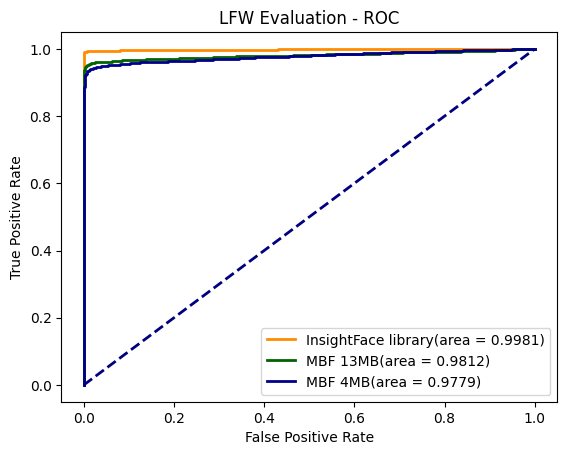
\includegraphics[width=0.5\linewidth]{images/compar.png}
  \caption{Đường cong ROC của các mô hình hiện thực trên máy tính đa dụng}
  \label{fig:roc}
\end{figure}

Với ngưỡng False Acceptance Rate (FAR) được cố định ở mức 3\% và 5\% trên tập LFW, độ chính xác và tỷ lệ từ chối nhầm của các cấu hình được trình bày trong Bảng \ref{tab:after_3} và Bảng \ref{tab:after_5}. Trong đó, kích thước của module được tính bằng tổng kích thước của mô hình trích xuất đặc trưng và mô hình phát hiện khuôn mặt, chưa bao gồm kích thước của các thư viện hỗ trợ.

\begin{table}[]
    \centering
    \small
    \begin{tabular}{|c|c|c|p{2.5cm}|p{2.5cm}|}
    \hline
      &\textbf{Model}  & \textbf{Size (MB)} & \textbf{ACC @FAR=5\% (\%)} & \textbf{FRR @FAR=5\% (\%)}\\
      \hline
      1&InsightFace library (baseline) & 12.9 + 2.4 = 15.3 &96.8333 & 0.5333 \\
      2&MobileFaceNet v13MB & 12.9 + 0.66 = 13.56&95.3582 & 3.8022 \\
      3&MobileFaceNet v4MB & 3.81 + 0.66 = 4.47&94.9714 & 5.0471 \\
      \hline
    \end{tabular}
    \caption{Bảng so sánh các chỉ số tại FAR=5\% khi hiện thực trên máy tính đa dụng}
    \label{tab:after_5}
\end{table}

\begin{table}[]
    \centering
    \small
    \begin{tabular}{|c|c|c|p{2.5cm}|p{2.5cm}|}
    \hline
      &\textbf{Model}  & \textbf{Size (MB)} & \textbf{ACC @FAR=3\% (\%)} & \textbf{FRR @FAR=3\% (\%)}\\
      \hline
      1&InsightFace library (baseline) & 12.9 + 2.4 = 15.3 &98.4333 & 0.6000 \\
      2&MobileFaceNet v13MB & 12.9 + 0.66 = 13.56&96.5691 & 4.0040 \\
      3&MobileFaceNet v4MB & 3.81 + 0.66 = 4.47&95.7787 & 5.4172 \\
      \hline
    \end{tabular}
    \caption{Bảng so sánh các chỉ số tại FAR=3\% khi hiện thực trên máy tính đa dụng}
    \label{tab:after_3}
\end{table}

Trong bài toán nhận diện khuôn mặt, tồn tại sự đánh đổi rõ rệt giữa độ chính xác và chi phí tài nguyên tính toán. Thư viện InsightFace, với độ chính xác gần như tối đa (AUC đạt 0.9981 và Equal Error Rate (EER) chỉ 0.0073), thể hiện khả năng phân tách rất tốt giữa các cặp khuôn mặt cùng và khác danh tính, do đó được sử dụng làm mô hình chuẩn (baseline) để so sánh trong đồ án.

Ở giai đoạn đầu, hệ thống sử dụng các biến thể của MobileFaceNet (MBF) với kích thước 13MB và 4MB, kết hợp với các thư viện nhẹ nhằm giảm thiểu phụ thuộc, đại diện cho kịch bản triển khai trên máy tính đa dụng. So với model pack của InsightFace, cấu hình đề xuất với sự kết hợp giữa MobileFaceNet và BlazeFace đạt được hiệu năng đáng chú ý với kích thước nhỏ gọn hơn:
\begin{itemize}
\item \textbf{MBF 13MB}: Sử dụng mô hình trích xuất đặc trưng của thư viện baseline, đạt AUC 0.9812. Mặc dù có sự suy giảm hiệu năng so với baseline, hệ thống đạt được mức giảm tương đối về kích thước (khoảng 2MB) nhờ thay thế mô hình phát hiện khuôn mặt.
\item \textbf{MBF 4MB}: Với kích thước chỉ 4MB, mô hình vẫn đạt AUC 0.9779. Đáng chú ý, khoảng cách hiệu năng giữa hai cấu hình trong đồ án nhỏ hơn so với khoảng cách tương ứng khi so sánh với baseline, cho thấy ảnh hưởng đáng kể của pipeline tiền xử lý và căn chỉnh khuôn mặt đối với chất lượng đặc trưng.
\end{itemize}

Kết quả thực nghiệm cho thấy, mặc dù các mô hình trong đồ án có tỷ lệ từ chối nhầm (False Rejection Rate – FRR) cao hơn so với baseline, mức chênh lệch này vẫn nằm trong ngưỡng chấp nhận được khi xét đến các ràng buộc phi chức năng của hệ thống. Điều này mở ra khoảng trống cho các bước nén tiếp theo nhằm tối ưu hóa tài nguyên. Bên cạnh đó, sự cải thiện rõ rệt từ Hình \ref{fig:before} sang Hình \ref{fig:roc} cho thấy vai trò quan trọng của các kỹ thuật tiền xử lý, đặc biệt là face alignment, trong việc nâng cao độ chính xác của hệ thống nhận diện khuôn mặt.
\subsection{Triển khai trên mạch ESP32-CAM}
\subsubsection{Nén mô hình}
Để đánh giá hiệu quả của các kỹ thuật nén, mô hình MobileFaceNet 4MB được sử dụng làm cấu hình cơ sở trong toàn bộ quá trình thực nghiệm.
\paragraph{Cắt tỉa mô hình} Quy trình iterative pruning kết hợp fine-tuning được thực hiện trên nền tảng Google Colab sử dụng PyTorch, với tập dữ liệu con được trích xuất từ CASIA-WebFace gồm 12.800 ảnh thuộc 718 danh tính. Quá trình tinh chỉnh được giám sát bởi hàm mất mát ArcFace với các tham số $s = 64$ và $m = 0.5$, nhằm duy trì khả năng phân tách trong không gian embedding. Việc huấn luyện sử dụng bộ tối ưu SGD với learning rate $1 \times 10^{-4}$, weight decay $1 \times 10^{-4}$ và momentum 0.9.

Do số lượng tham số của lớp depthwise convolution nhỏ hơn đáng kể so với lớp tích chập $1\times1$ (lần lượt là $9 \times t \times k$ so với $k \times t \times k$, với $k \geq 64$), quá trình cắt tỉa có cấu trúc (structured pruning) được tập trung chủ yếu vào các lớp $1\times1$ convolution. Bên cạnh đó, chiến lược cắt tỉa được phân bổ không đồng đều theo chiều sâu của mạng, trong đó ưu tiên các lớp trung gian nhằm hạn chế mất mát thông tin ở các lớp đầu vào, đồng thời vẫn đảm bảo khả năng phục hồi biểu diễn ở các lớp phía sau thông qua fine-tuning. 

\begin{figure*}
    \centering
    \begin{subfigure}[t]{0.45\textwidth}
        \centering
        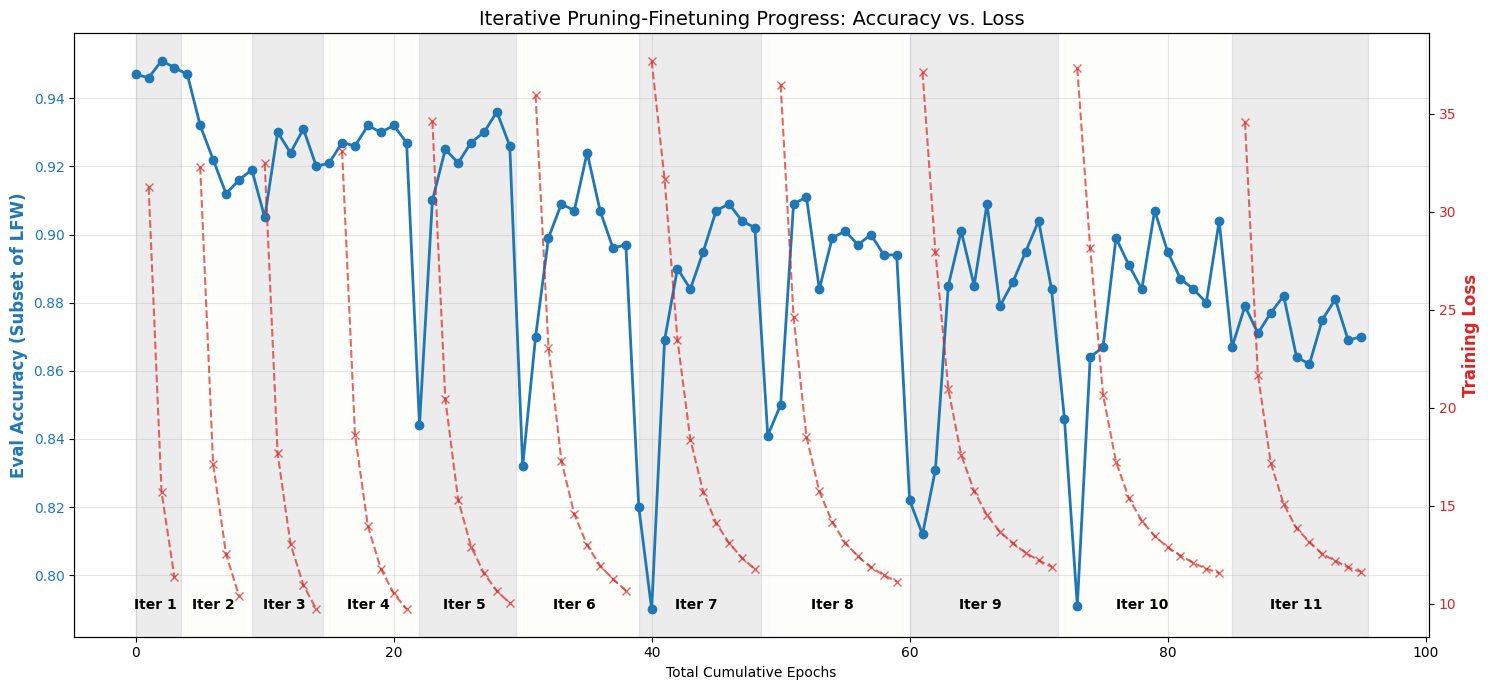
\includegraphics[width=\linewidth]{images/pruningg.png}
        \caption{Structured kết hợp unstructured pruning (Iter 11). Độ thưa thu được là 0.2 và 0.36}
        \label{fig:struct-unstruct-pruning}
    \end{subfigure}%
    ~
    \begin{subfigure}[t]{0.45\textwidth}
        \centering
        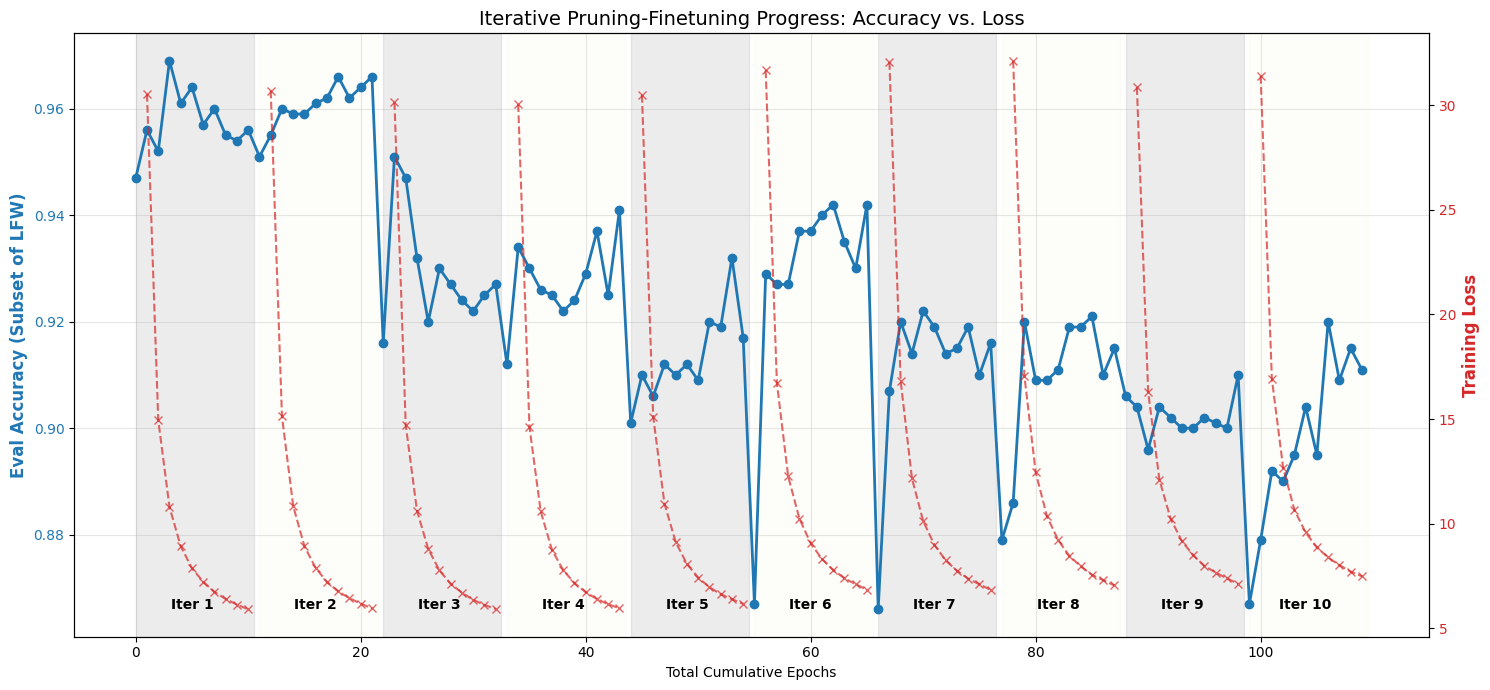
\includegraphics[width=\linewidth]{images/prune-015.png}
        \caption{Structured pruning. Độ thưa thu được là 0.15}
        \label{fig:struct-pruning}
    \end{subfigure}
    \caption{Quá trình iterative pruning - fine-tuning}
    \label{fig:pruning-finetuning}
\end{figure*}

Trước khi áp dụng cắt tỉa, mô hình cơ sở (MobileFaceNet 4MB) đạt hiệu suất tốt trên tập con của LFW, với độ chính xác đạt 95.87\%. 

Hệ thống sẽ được cắt tỉa ban đầu bởi các hàm trong thư viện PyTorch, bao gồm \texttt{torch.nn.utils.prune.ln\_structured} cho structured pruning và \texttt{torch.nn.utils.} \texttt{prune.global\_unstructured} cho unstructured pruning. Quá trình này được hiện thực thông qua việc áp dụng các mask lên trọng số của mô hình, cho phép vô hiệu hóa các tham số kém quan trọng mà không làm thay đổi trực tiếp cấu trúc dữ liệu ban đầu.

Để đánh giá ảnh hưởng của structured pruning, unstructured pruning và quá trình fine-tuning lên hiệu năng mô hình, hai kịch bản thực nghiệm được thiết kế. Trong kịch bản thứ nhất, mô hình lần lượt trải qua các bước iterative structured pruning và global unstructured pruning, qua đó thu được hai phiên bản mô hình với độ thưa tương ứng là 20\% và 36\% sau mỗi giai đoạn. Kết quả thực nghiệm của kịch bản được trình bày ở Hình \ref{fig:struct-unstruct-pruning}

Trong giai đoạn 1 (cắt tỉa có cấu trúc với mục tiêu 20\%), tại mỗi bước cắt tỉa, ngay sau khi loại bỏ các tham số, hàm mất mát huấn luyện (train loss) tăng đột biến lên mức cao (dao động trong khoảng 31.0–37.0). Tuy nhiên, nhờ quá trình fine-tuning, hàm mất mát giảm dần và hội tụ về khoảng 9.0–12.0 sau vài epoch. Điều này cho thấy cơ chế tinh chỉnh hoạt động hiệu quả, cho phép các tham số còn lại thích nghi nhằm bù đắp cho phần thông tin đã bị loại bỏ. Khi độ thưa tăng từ 0.02 lên 0.08, độ chính xác trên tập con LFW có xu hướng giảm dần nhưng vẫn duy trì ở mức ổn định. Tuy nhiên, từ ngưỡng khoảng 8\%, quá trình cắt tỉa bắt đầu gây ra sự suy giảm rõ rệt hơn về độ chính xác; mặc dù vậy, fine-tuning vẫn giúp phục hồi tốt một phần hiệu năng sau mỗi vòng lặp.

Ở bước tiếp theo, khi áp dụng global unstructured pruning, mức suy giảm độ chính xác quan sát được thấp hơn so với các bước structured pruning trước đó. Tuy nhiên, khả năng phục hồi thông qua huấn luyện lại là hạn chế, mặc dù train loss giảm đáng kể (từ 34.57 xuống 11.61). Hiện tượng này cho thấy mô hình đã vượt qua “ngưỡng chịu đựng”, khi việc loại bỏ khoảng 36\% tham số đã làm mất đi nhiều đặc trưng quan trọng (critical weights) mà phần còn lại không thể bù đắp.

Trong kịch bản thứ hai, hệ thống chỉ áp dụng structured pruning với 10 vòng lặp (iterations) nhằm đạt độ thưa mục tiêu 15\%. Kết quả cho thấy mô hình đạt độ chính xác trên tập LFW là 91.52\%, phù hợp với những gì quan sát được ở kịch bản đầu tiên. Diễn biến của quá trình huấn luyện được minh họa trong Hình \ref{fig:struct-pruning}.

\begin{figure}[ht]
\centering
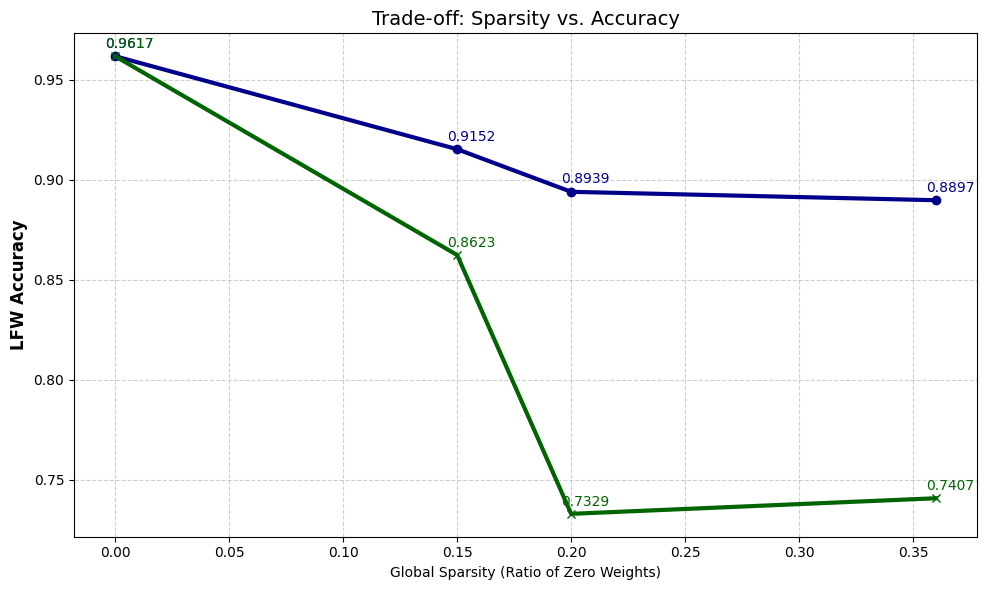
\includegraphics[width=0.8\linewidth]{images/before-after.png}
\caption{Độ chính xác của mô hình ở các mức thưa khác nhau, trước và sau sử dụng torch-pruning.}
\label{fig:real-prune}
\end{figure}

Tuy nhiên, với cơ chế cắt tỉa trong thư viện PyTorch, các trọng số sau khi bị loại bỏ vẫn được lưu trữ dưới dạng ma trận dày đặc (dense tensors) thông qua cơ chế masking hoặc được merge lại trên ma trận trọng số mà không thay đổi kích thước của các tensor. Do đó, kích thước mô hình và số phép toán (MFLOPs) không thay đổi mặc dù độ thưa đã tăng.

Để thực sự giảm kích thước mô hình, thư viện torch-pruning\cite{fang2023depgraph} được sử dụng nhằm phân tích đồ thị phụ thuộc (dependency graph), loại bỏ hoàn toàn các kênh có giá trị bằng 0 và các kênh liên quan. Do tính chất phụ thuộc giữa các lớp, việc cắt tỉa một lớp sẽ kéo theo điều chỉnh cấu trúc ở các lớp liên quan, dẫn đến sự suy giảm đáng kể về độ chính xác (Hình \ref{fig:real-prune}). Tuy nhiên, đổi lại, kích thước mô hình và số phép toán đã được giảm đáng kể. Các chỉ số chi tiết của các mô hình sau khi áp dụng torch-pruning được trình bày trong Bảng \ref{tab:prune-table}.

\begin{table}[]
\centering
\small
\begin{tabular}{|l|c|c|c|c|c|}
\hline
\textbf{Độ thưa} & \textbf{Kích thước (MB)} & \textbf{Params} & \textbf{FLOPs (G)} & \textbf{LFW ACC (\%)} & \textbf{FRR@FAR=5\%}\\
\hline
0.0  & 3.8 & 1.013M & 0.227 & 96.17 & 5.047\\
0.15 & 3.2 & 0.848M & 0.193 & 86.2 & 24.125\\
0.2 & 3.1 & 0.811M & 0.186 & 73.3 & 56.830\\
0.36 & 3.1 & 0.811M & 0.186 & 74.1 & 57.470 \\
\hline
\end{tabular}
\caption{Bảng so sánh các chỉ số của mô hình MobileFaceNet v4MB sau khi cắt tỉa}
\label{tab:prune-table}
\end{table}

Dựa trên kết quả thực nghiệm trong Bảng \ref{tab:prune-table}, có thể quan sát rõ sự đánh đổi giữa hiệu năng tính toán và độ chính xác của mô hình khi áp dụng các kỹ thuật cắt tỉa khác nhau.

Khi tăng dần độ thưa của mô hình, các chỉ số liên quan đến tài nguyên tính toán đều được cải thiện đáng kể. Cụ thể, tại mức độ thưa 0.15, số lượng tham số giảm khoảng 16.3\% (từ 1.013M xuống 0.848M), trong khi số phép toán FLOPs giảm khoảng 14.98\% (từ 0.227G xuống 0.193G). Điều này cho thấy phương pháp structured pruning kết hợp với torch-pruning đã loại bỏ hiệu quả các kênh dư thừa, qua đó giảm khối lượng tính toán và kích thước thực tế của mô hình. Tuy nhiên, kết quả cũng cho thấy sự suy giảm đáng kể về độ chính xác sau khi thực hiện physical pruning. Cụ thể, độ chính xác giảm khoảng 5.29\% tại mức độ thưa 0.15 và giảm mạnh hơn, khoảng 14.9–16.1\%, tại các mức độ thưa 0.2 và 0.36. Điều này cho thấy khi độ thưa vượt quá một ngưỡng nhất định, các tham số bị loại bỏ không còn chỉ là các trọng số dư thừa mà đã bắt đầu ảnh hưởng trực tiếp đến các đặc trưng cốt lõi phục vụ cho bài toán phân biệt khuôn mặt.

Đối với ảnh hưởng của structured pruning và unstructured pruning, kết quả thực nghiệm cho thấy sự khác biệt rõ rệt về hiệu quả thực tế. Trong khi mức độ thưa 0.15 mang lại sự giảm đáng kể về số lượng tham số và FLOPs - đặc trưng của structured pruning - thì từ mức độ thưa 0.2 đến 0.36, các chỉ số vật lý như kích thước mô hình (3.1 MB) và FLOPs (0.186G) hầu như không thay đổi. Hiện tượng này phản ánh bản chất của unstructured pruning, trong đó các trọng số riêng lẻ bị đưa về 0 nhưng cấu trúc tensor và kích thước các lớp vẫn được giữ nguyên. Do đó, nếu không có phần cứng hoặc thư viện hỗ trợ tính toán ma trận thưa chuyên dụng, phương pháp này khó mang lại lợi ích đáng kể về tốc độ suy luận hoặc mức sử dụng bộ nhớ trên các nền tảng nhúng tiêu chuẩn.

Ngoài ra, khi tăng độ thưa từ 0.2 lên 0.36 bằng global unstructured pruning, độ chính xác trên tập LFW chỉ thay đổi nhẹ (từ 73.3\% lên 74.1\%). Sự chênh lệch nhỏ này có thể đến từ nhiễu thực nghiệm hoặc ảnh hưởng của quá trình fine-tuning sau cắt tỉa. Tuy nhiên, xét tổng thể, cả hai mô hình đều đã rơi vào trạng thái suy giảm hiệu năng nghiêm trọng so với mô hình gốc.

Từ các kết quả trên có thể thấy rằng, mặc dù unstructured pruning cho phép đạt mức độ thưa cao hơn, phương pháp này không mang lại lợi ích thực tế tương ứng về chi phí tính toán và kích thước mô hình trong bối cảnh triển khai trên thiết bị nhúng. Ngược lại, structured pruning ở mức độ thưa khoảng 0.15 cho thấy sự cân bằng hợp lý hơn giữa hiệu năng và tài nguyên, phù hợp hơn cho các hệ thống có giới hạn nghiêm ngặt về bộ nhớ và năng lực tính toán như ESP32.

\paragraph{Lượng tử hóa mô hình}
Tiếp tục sử dụng phiên bản mức độ thưa 0.15 (MobileFaceNet v4MB p0.15)
\subsubsection{Hiện thực chương trình}
\subsubsection{Kết quả đạt được}
\subsection{Tích hợp với hệ thống HealthKiosk}
\section{Đánh giá hiệu năng hệ thống}


\subsection{So sánh giữa các mức độ nén}
\subsection{Đánh giá toàn diện trên máy tính đa dụng}
\subsection{Đánh giá toàn diện trên thiết bị nhúng}


